\documentclass[conference]{IEEEtran}

\newcommand{\thetitle}{An Atomic Theory of Flow Behavior}

\usepackage[pdftex]{graphicx}
\usepackage[labelfont=bf,small]{caption}
\usepackage[font=small,labelfont=bf,position=top,nearskip=0em]{subfig}
\usepackage{cite,amsmath,amssymb,rotating,multirow,bigstrut,url,wrapfig}
\usepackage[hyperfigures,bookmarks,bookmarksopen,bookmarksnumbered,frenchlinks=true,pdftitle={\thetitle}]{hyperref}

\hyphenation{op-tical net-works semi-conduc-tor IEEEtran}
\bibliographystyle{IEEEtran}

\newcommand{\email}[1]{$\left<{\textit{#1}}\right>$}
\newcommand{\caps}[1]{{\small{#1}}}

\title{
\vspace{-0.25em}
\thetitle
}
\author{
{\large{Stefan~Karpinski, Elizabeth~M.~Belding, Kevin~C.~Almeroth}} \vspace{0.25em}\\
Department of Computer Science \\
University of California, Santa Barbara \vspace{0.35em}\\
\textit{\{sgk,ebelding,almeroth\}@cs.ucsb.edu}
%\vspace{-0.5em}
}

\newcommand{\todo}[1]{[\textit{\textbf{TODO}: {#1}}]}

\newcommand{\E}[1]{\left<#1\right>}
\newcommand{\abs}[1]{\left|#1\right|}
\newcommand{\R}{\mathbb{R}}
\newcommand{\Z}{\mathbb{Z}}
\newcommand{\N}{\mathbb{N}}
\newcommand{\Q}{\mathbb{Q}}
\newcommand{\ceil}[1]{\left\lceil#1\right\rceil}
\newcommand{\floor}[1]{\left\lfloor#1\right\rfloor}

\newcommand{\figurename}{Figure}
\newcommand{\tablename}{Table}

\renewcommand{\topfraction}{0.95}% max fraction of floats at top
\renewcommand{\bottomfraction}{0.95}% max fraction of floats at bottom
\setcounter{topnumber}{4}
\setcounter{bottomnumber}{4}
\setcounter{totalnumber}{4}% 2 may work better
\setcounter{dbltopnumber}{4}% for 2-column pages
\renewcommand{\dbltopfraction}{0.9}	% fit big float above 2-col. text
\renewcommand{\textfraction}{0.07}% allow minimal text w. figs
\widowpenalty=1000
\clubpenalty=1000

\graphicspath{{plots/}}

\begin{document}
\maketitle

\begin{abstract}
We propose an entirely new approach to understanding and analyzing the behavior of flows in packet networks. The essential concept of this new approach is to find atomic units of time and size behavior in traces of network flows. While the nonparametric statistical techniques for extracting these basic behavioral units are complex, the end result is quite simple: the units provide an alphabet for flow behavior. From a finite set of behavioral units, an infinite variety of actual behaviors can be composed. The space of behaviors naturally becomes a vector space generated by these atomic units of behavior. We use numerical linear algebra techniques to demonstrate useful and immediate applications of this theory to real-time traffic analysis, anomaly and attack detection, as well as workload generation for wireless experiments.
\end{abstract}

\section{Introduction}\label{sec:intro}

The trouble with trying to understand or model behavioral patterns in packet networks is that beyond the packets themselves there is no inherent behavioral structure. There are flows of packets with the same source and destination \caps{IP} addresses and \caps{TCP/UDP} port numbers, and sessions of flows belonging to the same host, but these imply only very limited behavioral similarity. Each one has its own unique sequence of packet sizes and inter-packet intervals with no obvious relation to each other. Without fundamentally behavioral elements of structure, traffic traces are just ``packet soup,'' so to speak. Accordingly, traditional approaches to traffic analysis have either focused on aggregate traffic measures or categorized flows by well-known port numbers and application types. Some fiendishly clever techniques have been proposed to tease out the applications types underlying traffic found in network traces~\cite{Karagiannis05}. Without an inherently behavioral theory of network traffic, however, we believe that insight into the fine structure of network behavior is ultimately very limited.

%Such indirect approaches, however, can ultimately provide only limited insight into the fine structure of network behavior.

We propose to turn this problem on its head by providing an atomic behavioral theory for network traffic. We begin with the concept of a packet flow as a natural starting point and define a ``{flowlet}'' as a segment of a flow with statistically consistent packet size or inter-packet interval behavior. %\footnote{The word ``or'' is not a typo: there are two independent types of flowets.}
Common flowlet behaviors are extracted from a body of traffic traces, using statistical clustering. These clusters of similarly behaved flowlets provide the atomic units of flow behavior: by mixing basic behaviors from a finite collection of flowlet clusters in varying proportions, an infinite variety of flow behaviors emerge. It becomes natural to view the space of flow behaviors as a vector space of linear combinations of flowlet clusters.

To demonstrate the viability and utility of this atomic theory of flow behavior, we apply standard numerical linear algebra techniques to the resulting vector space of flow behaviors. Principal component analysis (\caps{PCA}) allows us to reduce the dimensionality of the vector space of flow behaviors while preserving the vast majority (99\%) of the variatibility in the original data. \caps{PCA} allows us to represent flow behaviors concisely in only eight dimensions ($\R^8$). Moreover, this representation has several desirable properties. The eight coordinates of flows mapped into this space are linearly uncorrelated (non-linear dependencies, however, remain). The first dimension of the transformed data captures the most important differences between flows; the second dimensions the next most important, and so on. The first two or three dimensions, thus, are ideal for visualization of behavioral differences. Finally, the dimensions are naturally scaled so that the standard Euclidean distance provides a good measure of the behavioral (dis)similarity between flows. As a result, standard multi-dimensional analysis and modeling techniques, such as $k$-means clustering, can be applied directly to the transformed flow behaviors.

We present two useful, immediate applications of this new theory of flow behavior. First, once a body of traffic has been analyzed and \caps{PCA}-transformation matrices computed, new flows can be mapped into the flow-behavior space using only fast matrix and vector computations with pre-computed matrices. This allows the possibility of completely real-time traffic analysis and visualization.
%
Second, since the coordinates of the \caps{PCA}-transformed flow behaviors are uncorrelated and exhibit limited non-linear dependencies, we can roughly model them using a multivariate normal distribution. Random deviates from this distribution can be mapped back into actual flow behaviors, allowing the generation of an entire network's worth of heterogeneous synthetic flow behaviors with the realistic intra-flow and inter-flow behavior matching the original trace traffic. This ability is of particular importance for experimental wireless research, where it has been shown that using standard, na\"ive traffic models, such as the uniform constant bit-rate (\caps{CBR}) flows, severely distorts important performance metrics at all levels of the network~\cite{Karpinski07:realism,Karpinski07:cbr-failure}.

%Three final characteristics make our analytical methodology particularly promising. First, the techniques and results are described are not dependent on the data we have used: they can be applied to any collection of network traffic. 

%, with the dimensions ordered to capture diminishing variance in behavior. Thus, the first two dimensions can be used to provide a faithful visual map of flow behaviors. Standard clustering techniques can be applied to the transformed data to discover behavioral similarities across protocol boundaries. Moreover, once the transformation has been established from real data, it can be quickly applied to new flows using simple matrix operations. Our methodology thereby allows for real-time analysis of network traffic.

%%Common flowlet behaviors are found across all the flows in network traces, thereby providing the basis for an atomic theory of flow behavior. 

%%We provide the statistical and computational techniques needed to extract flowlets from traffic traces, we provide the basic building blocks for understanding flow behavior.

%%What we propose is a view of network traffic that let's us directly characterize the \textit{behavior} of flows, and then view the traditional traffic types as annotations to that fundamental characterization. 

%% How can one even begin to analyze flow behavior data, when each flow has a completely unique signature of packet sizes and inter-packet intervals. The first part of our analysis methodology addresses this problem by extracting ``atoms'' of flow behavior. First we split each flow into segments of homogeneous behavior, and then we cluster these segments across all the flows to find elements of similar behavior from which all flows are composed. You can think of these clusters an alphabet for flow behavior: flows are words composed by stringing together sequences of letters.

%Traffic patterns in wireless local-area networks (\caps{WLAN}s) have recently become recognized as a subject of significant interest and importance in wireless research~\cite{Papadopouli05,Hernandez06:wlan-traffic,Ploumidis07,Karaliopoulos07,Karpinski07:realism,Karpinski07:cbr-failure}. It has been shown that using common, na\"ive traffic models in experiments can severely distort important performance metrics at all levels of the network, sometimes completely inverting relative performance of protocols~\cite{Karpinski07:cbr-failure}. Significant progress has been made in understanding and modeling the high-level properties of traffic patterns in \caps{WLAN}s~\cite{Papadopouli05,Hernandez06:wlan-traffic,Ploumidis07,Karaliopoulos07}. Finding complete multi-level traffic models that can accurately reproduce the performance characteristics of real-world traffic, however, remains an unsolved problem.

%% Understanding and modeling the complete pattern of traffic in any local-area network is an extremely challenging analytical modeling problem. Transmissions in the network are logically organized into flows, consisting of series of packets between a pair of nodes on a fixed pair of \caps{TCP} or \caps{UDP} port numbers. Thus, each flow is already a related pair of time series, whose behavior can exhibit complex feedback. The network is comprised of a many nodes with heterogeneous behavioral characteristics, and with a vast variety of flows connecting them. The flows themselves are described by distributions of packet sizes and inter-packet intervals, but across the entire collection of flows and nodes, one finds distributions of these distributions. In short, the ``curse of dimensionality'' which plagues so many modeling problems appears in spades.

%%\todo{discuss challenges and applications}

%In this paper we use a series of advanced statistical techniques to analyze, understand, and visualize the space of packet size and inter-packet interval distributions found in real-world \caps{WLAN} traffic. Our work complements the top-down approach that most research in this area has taken. In particular, the work of Hern\'andez-Campos~\textit{et~al.} provides high-level session and flow models that give a convincing overview of network traffic. Karpinski~\textit{et~al.}~\cite{Karpinski07:realism} showed that if, in addition to such high-level models, the distributions of packet sizes and inter-packet intervals across all flows can be realistically modeled, then whole-network performance characteristics can be accurately reproduced in simulation.

%Reproducing a network's worth of heterogeneous flow behaviors in a manner that resembles reality is easier said than done, however. The multi-level complexity, non-linear feedback, and the very high dimensionality of the spaces involved conspire to make the analysis seem all but intractable. In the last decades, however, a great deal of work has been done in fields with similar difficulties: biometrics, econometrics, genetics, ecology, meteorology. The common tools of these fields, when traditional methods fail, are nonparametric statistics, clustering, and a variety of dimensionality reduction techniques. We employ all of these to extract order from the chaos of network flow behavior.

%Our processing methodology transforms raw trace data through a series of stages such that common structure is extracted at every stage, while each flow's individual behavior can still be reconstructed without significant loss of accuracy. %\footnote{Our threshold for loss of accuracy at each transformation is 1\%. We use a standard significance level of $\alpha=0.05$ for our statistical tests.}
%In overview, the procedure first uses time series change point detection to extract basic elements of time and size behavior from raw flow data. Each flow is split into ``flowlets''---sequences of packets with homogeneous statistical behavior. The flowlets are then clustered across flows, extracting common elements of behavior for the entire data set. Finally, we apply standard numerical linear algebra techniques to further reduce the dimensionality of the representation, until each flow can  be expressed with only eight real-valued coefficients.

%The transformed representation of flow behaviors has many useful properties. The coordinates of the transformed data are uncorrelated and normalized, with the dimensions ordered to capture diminishing variance in behavior. Thus, the first two dimensions can be used to provide a faithful visual map of flow behaviors. Standard clustering techniques can be applied to the transformed data to discover behavioral similarities across protocol boundaries. Moreover, once the transformation has been established from real data, it can be quickly applied to new flows using simple matrix operations. Our methodology thereby allows for real-time analysis of network traffic.

%Finally, since the coefficients of the transformed flows are guaranteed to be uncorrelated with zero mean---and because they happen to exhibit limited dependence---we can roughly approximate their distribution as a standard multivariate normal. Random deviates of this approximating distribution can be transformed back into flow behaviors, allowing us to randomly generate collections of flows in a more realistic manner than has previously been achieved.

%%The rest of the paper is organized as follows. In Section~\ref{sec:motivation} we present motivation and related work. Our analytical methodology is presented in Section~\ref{sec:methodology}, while the results of our experiments are explained and analyzed in Section~\ref{sec:results}. Finally, in Section~\ref{sec:conclusions}, we conclude with the impact of and future directions for this research.

%%This work is a collection of advanced analytical techniques for exploring and understanding the fine structure of flow behavior across a large body of traffic. The specific results are of less importance than the techniques themselves, which are far from obvious, and can be applied to many different data sets---and even in other domains.

\section{Motivation \& Related Work}
\label{sec:motivation}
\label{sec:related-work}

In Internet traffic analysis, the detailed structure of workload patterns in local-area networks (\caps{LAN}s) is of limited interest. 
%Bottlenecks in the Internet are found in the core of the Internet or at the last mile.
Capacity has become so cheap and plentiful in wired \caps{LAN}s that workload details are simply irrelevant in the face massive over-provisioning. Wireless networks, however, are fundamentally different: the entire medium is at the ``edge'' of the network and the most basic resources of bandwidth and power are severely limited, with no permanent relief in sight. Thus, over-provisioning is simply not an option, and the fine-grained details of traffic patterns have been shown to have a dramatic impact on network performance~\cite{Karpinski07:realism,Karpinski07:cbr-failure}.
As a result, modeling and analysis of wireless \caps{LAN} (\caps{WLAN}) traffic has recently become a hot topic in the wireless community, and a significant body of high-quality research on this subject has been produced~\cite{Papadopouli05,Hernandez06:wlan-traffic,Ploumidis07,Karaliopoulos07,Karpinski07:realism,Karpinski07:cbr-failure}.

Most of the recent surge of research in \caps{WLAN} traffic has taken a top-down approach, using parametric models to reproduce high-level statistical characteristics of observed workload behavior~\cite{Papadopouli05,Hernandez06:wlan-traffic,Ploumidis07,Karaliopoulos07}. In particular, Her\'andez-Campos~\textit{et~al.}~\cite{Hernandez06:wlan-traffic} showed convincingly that the following models are applicable to \caps{WLAN} traffic: user arrivals (sessions) follow a time-varying Poisson model; the number of flows per session follows a BiPareto distribution; the sizes of flows follow a BiPareto distribution; the intervals between the initiations of flows within each session follow a Lognormal distribution. These models provide an excellent and convincing high-level overview of the behavior of users and applications in \caps{WLAN}s.

The methodology for generating synthetic workload remains incomplete, however. While the high-level scaffolding for producing \caps{WLAN} traffic exists, the low-level behavior of flows is neither understood nor reproducible. The common practice in workload generation is to use a uniform constant bit-rate (\caps{CBR}) model for the packet-level behavior of flows: all flows have the same number of packets, all packets have identical size, and the intervals between packets in each flow are of a single, fixed duration. % TODO: citation describing CBR
Karpinski~\textit{et~al.}~\cite{Karpinski07:cbr-failure}, however, showed that all types of \caps{CBR} packet behavior models drastically distort important performance metrics, and thus fail the litmus test for realism. Distorted performance resulted even when \caps{CBR} was applied with high-level behavior taken directly from traces \textit{and} using accurate packet count, average packet size, and average inter-packet interval for each flow~\cite{Karpinski07:realism}.% More sophisticated models of packet-level flow behavior are needed before accurate simulation results can be achieved.
%Moreover, in this work, it was assumed that not only how many packets each flow consisted of, but also the total duration of each flow, and thus its average data rate, were both accurately modeled. While this research did not specifically examine the mixed-model case where only one of these parameters was known, this additional ignorance can only worsen the accuracy the model.

Using variable bit-rate (\caps{VBR}) flows is a common elaboration upon the \caps{CBR} flow model. In \caps{VBR} models, the packets sizes and the inter-packet intervals are each randomly sampled from pre-specified, independent, identically distributed (i.i.d.) distributions. % TODO: citation for VBR
% independently randomly sampled from fixed, pre-specified distributions. %Both the packet sizes and inter-packet intervals are thus modeled as separate, independent and identically distributed (i.i.d.) time series.
One of the most significant results of~\cite{Karpinski07:realism} is that if high-level workload is realistic, then an i.i.d. \caps{VBR} model for flow behavior accurately reproduces network performance---with one \textit{very} major caveat: each flow must have its own unique, realistic signature of packet size and inter-packet interval distributions. Producing a realistic cross-network collection of these distributions is, to date, an unsolved problem. The size and interval distributions used in~\cite{Karpinski07:realism} were empirical estimates, taken directly from the observed behavior of each flow in the original trace. This result has a very important implication for the present work: \textit{to characterize flow behavior, it is sufficient to know each flow's distribution of packet sizes and inter-packet intervals}. It is precisely this problem of understanding, modeling, and recreating realistic collections of packet size and inter-packet interval distributions for an entire network that this paper addresses.

% This requirement, however, is non-trivial to satisfy. The size and interval distributions used in~\cite{Karpinski07:realism} were not simple parametric distributions typically used with \caps{VBR} models. Rather, they were empirical distributions taken directly from the observed behavior of each flow in the original trace. Thus, every flow has a unique signature of packet sizes and inter-packet intervals. To produce a realistic \textit{collection} of such signatures, requires an understanding of what realistic signatures ``look like,'' and how frequently they occur relative to each other.

%The work of Hern\'andez-Campos~\textit{et~al.} has provided a statistically validated high-level framework for \caps{WLAN} traffic patterns. Karpinski~\textit{et~al.} demonstrated that given such a high-level framework, together with realistic per-flow packet size and inter-packet interval distributions, one can produce a complete and sufficiently realistic model for generating \caps{WLAN} traffic. In this research we address the outstanding problem: understanding and modeling the packet size and inter-packet interval distributions of flows in a \caps{WLAN}. 

%There are still, however, some rather large gaps in this picture. Because the various distributions are sampled independently, it follows that both the collections flows of each for user/session, and their individual packet-level behaviors, on average, look alike. Intuitively, on the other hand, it seems clear that different users must have different basic flow- and packet-level behaviors. It remains an open question whether this intuitively unrealistic uniformity of flow and packet behavior affects important performance characteristics. The methodology we introduced in~\cite{Karpinski07:realism} and made statistically rigorous in~\cite{Karpinski07:cbr-failure} promises the ability to shed light on this question.

%One of the open questions is whether these distributions can all be sampled independently. It may be that there is correlation between the per-user flow count value and the sizes or inter-arrival times of the individual flows.

%Another open problem is how to generate individual packets for each flow. Our previous work~\cite{Karpinski07:cbr-failure} showed that the constant bit-rate \caps{CBR} packet behavior model, even when employed with higher level behavior taken directly traces, still fails to accurately reproduce all of the performance metrics considered, except for average end-to-end network latency. Even in the ``good'' case of average end-to-end latency, factor of error induced by the \caps{CBR} model exceeded a factor of two half or the time! Moreover, this model assumed that it was known, not only how many packets each flow consisted of, but also the total duration of each flow, and thus its average data rate. While we did not examine the mixed-model case where only one of these parameters was known, this additional ignorance can only worsen the accuracy the model.

%Our work complements this by providing an objective, rigorous methodology for measuring how accurately synthetic models reproduce the performance characteristics of real-world traffic~\cite{Karpinski07:realism,Karpinski07:cbr-failure}. This paper aims to bridge the gap by 

%Previous work has shown that with knowledge of the following properties for each flow, realistic performance of wireless traffic can be reproduced accurately:
%\begin{enumerate}
%\item packet count (equivalently, duration),
%\item distribution of packet sizes,
%\item distribution of inter-packet intervals.
%\end{enumerate}
%In short, for the purpose of generating experimental workload that accurately predicts performance under real-world traffic conditions, it is sufficient to know the marginal distributions of packet properties, without any time series analysis. Each simulated flow can be produced by generating a sequence of packets in the following manner: randomly generate a packet size by sampling the size distribution; wait a randomly generated duration sampled from the inter-packet interval distribution; repeat until the appropriate number of packets has been generated.

\section{Methodology}
\label{sec:methodology}

Our goal is to provide an effective general methodology for analyzing and characterizing the space of packet size and inter-packet interval distributions found across the flows in \caps{WLAN} trace traffic. In essence, we require a ``distribution of distributions.'' %Essentially, one needs to find the subspace of all possible signatures in which realistic signatures occur, and how often.
However, size and interval distributions exist in spaces with very high dimensionality. In theory, both types of distributions live in infinite-dimensional Hilbert spaces. %TODO: verify this
%\footnote{The space of size distributions has a countably infinite number of dimensions, while the space of inter-packet interval distributions has an uncountably infinite number of dimensions.}
In practice, limits on possible values and quantization make the effective dimensions finite, but nonetheless too large for simple, direct analysis.% of the regions in which realistic flow behaviors can be found.

%\todo{paragraph about data}

To reduce the dimensionality of distribution data, we use a series of techniques.
First, we divide each flow's sequence of values---sizes or inter-packet intervals---into segments of consistent behavior, using time series change point detection. We call these segments of flows ``flowlets.'' Second, we apply agglomerative clustering to find clusters of flowlets with mutually consistent behaviors. These flowlet clusters are the atomic units that allow us to systematically apply standard techniques from other fields to analyze and understand flow behaviors. Each flow's behavior can be expressed as some weighted sum of constituent flowlet clusters. Thus, the space of flow behaviors have naturally become a vector space generated by the flowlet clusters. In the final stage of processing we use principal component analysis (\caps{PCA}) to reduce dimensionality of this vector space and isolate the most important aspects of behavior across the entire collection.

%The resulting transformation allows us to meaningfully represent the space of flow behavior in only a small number of dimensions (in our case, eight). Even more importantly, the transformation captures the vast majority (99\%) of the variations in flow behavior. Finally, the transformed data can be roughly approximated by a multi-variate normal distribution, and random deviates of this distribution can be mapped back into the original space of flow behaviors. This provides a way to generate collections of random flow behaviors such that the relationships and patterns found in the trace are respected and preserved.
% with respect to packet size or inter-packet intervals in one, two or three dimensions. With each additional dimension, more information about the behavior is captured. %Finally, we analyze the geometry and distribution of behaviors with respect to their principal components.

%Using clustering followed by \caps{PCA} is a common approach to analyzing data with high-dimensionality. % TODO: cite this
%The nature of our data, however, requires novel techniques---these are not standard multidimensional data-points for which normal clustering techniques or standard \caps{PCA} can be utilized. Rather, the data are variably sized samples from unknown, nonparametric distributions. Our clustering and \caps{PCA} methods are specially designed, based on prior art in nonparametric statistics, to address the difficulties encountered in this problem.

\subsection{Nonparametric Goodness-of-Fit Tests}

%It was demonstrated experimentally in~\cite{Karpinski07:realism} that it suffices to know the high-level behavior and the marginal distributions of packets sizes and of inter-packet intervals for each flow, to reproduce realistic performance characteristics in simulation. This implies that these two distributions together adequately characterize the packet-level behavior of the flow. %These distributions come from the actual collection of packets sent and received at wireless nodes in a \caps{WLAN}.

%The first step in analyzing packet-level flow behavior is determining essential similarities and differences within and across flows. When does the behavior of a single flow change from one ``mode'' to another? When can the behaviors of two different flows be considered to be the same? 
%To answer these questions, we turn to the statistical technique of goodness-of-fit testing. A goodness-if-fit test determines how likely it is that a sample came from a given distribution, or more generally, how likely it is that two samples came from the same distribution.

In the case of packet sizes and inter-packet intervals, there are no ``clean'' parametric models that capture the variety of behaviors seen in network traces. Therefore, we rely on nonparametric statistical procedures for our analysis. There are a number of nonparametric two-sample goodness-of-fit tests in the statistical literature. % TODO: citation here
Such tests take two samples of scalar values and test the null hypothesis that the samples were drawn from the same (unknown) underlying distribution. Nonparametric tests do not make any assumptions about the shape or nature of the underlying distributions, other than that they are continuous and real-valued. Such tests can detect various differences in both location and shape of distributions. We use the Baumgartner-Wei\ss-Schindler (\caps{BWS}) test~\cite{Baumgartner98} rather than the more well-known Kolmogorov-Smirnov (\caps{KS}) or Cram\'er-von Mises (\caps{CvM}) tests because: \caps{BWS} exhibits significantly superior power in simulation; the exact distribution of the \caps{BWS} test statistic for small sample sizes is already very close to its asymptotic distribution, which is untrue for \caps{KS} and \caps{CvM}.

% First, the \caps{BWS} test is experimentally more powerful for detecting differences in both location and shape, performing very nearly as well as parametric tests, in cases where such specialized tests exist.\footnote{There is a generalized CvM-type two-sample test~\cite{Pettitt79} that may compare more favorably with the BWS test. However, no simulated results were presented by which to evaluate its power. This generalized CvM and BWS are closely related: both use the same variance-weighted CvM integral as their basis, but apply different estimators of this integral as test statistics.} Second, in certain cases both the \caps{KS} and \caps{CvM} tests suffer from limited power as sample size grows: even when the sample size is allowed to go to infinity, the test power can level off well before reaching unity. This causes many failures to reject the null hypothesis even when samples are large and significant underlying differences exist. The \caps{BWS} test does not exhibit this effect. Finally, the exact distribution of the \caps{BWS} statistic approaches its asymptotic distribution very quickly: the asymptotic distribution is already a good approximation for samples as small as ten values. This is highly desirable since the cost of computing exact distributions grows exponentially with sample size, so the asymptotic distribution must be used even for modestly sized samples.

%These sets of values for packet size and inter-packet intervals can be considered as a sample from the underlying behavioral distributions for each flow. When asking the question of whether two flows have the same fundamental behavior, we are presented with a statistical dilemma: \textit{how likely is it that these two samples were randomly drawn from the same underlying distribution}.

\subsection{Flow Splitting}\label{sec:flow-splitting}

The first analytical task is to split the packet size and inter-packet interval time series for each flow into segments with consistent statistical behavior. A great deal of classical statistical research has been done in the general area of time series change point detection~\cite{Basseville93}. These classical approaches, however, cannot be applied when the number of change points are unknown and, worse still, the underlying models for the stochastic processes are unknown. Work has been done in econometrics that allows a single change point to be discovered using nonparametric \caps{KS} or \caps{CvM} type significance tests~\cite{Inoue01}. Zheng~\textit{et~al.}~\cite{Zhang01} use recursive iteration of this procedure with the Fligner-Policello (\caps{FP}) test to detect change points in Internet path properties. Our technique is the same except that we use the \caps{BWS} test rather than \caps{FP}; the \caps{FP} test detects only changes in central location, whereas \caps{BWS} detects changes in both location and shape.%
\footnote{Our ``backward elimination'' post-processing procedure differs slightly too: we eliminate the least significant change point candidate first and iterate until only significant ones remain; Zhang~\textit{et~al.} eliminate insignificant candidates in sequential order. In cases where these procedures produce different results, our algorithm yields more homogeneous behavior between change points.} %We also stop our recursion if either the left or right sets of values becomes smaller than ten. At this point statistical tests lose power, and can easily suffer from both false rejections of the null and false failures to reject the null.
Allen~\textit{et~al.}~\cite{Allen07} use this procedure with the \caps{KS} test to detect change points in time series of network bandwidth measurements.
Space unfortunately does not permit us to reproduce the procedure here.
%We briefly describe the procedure here.
%
%\subsubsection{Candidate Generation}
%For each sequence index, $k$, compute the $p$-value comparing the set of values to the left of $k$ compared with the set of values to the right of $k$. Split the sequence at the value of $k$ with the most significant (smallest) $p$-value and recurse. Terminate the recursion if either half is empty or if none of the $p$-values are significant. Each splitting point is a candidate change point for the second phase.
%
%\subsubsection{Candidate Elimination}
%Iterate through set of candidate change points, computing the $p$-value of the samples of values immediately before and after each candidate (i.e. with no intervening candidates). Of the candidates that are insignificant, eliminate the one with the least significant (largest) $p$-value and iterate. Terminate the iteration when all $p$-values are significant. The remaining candidates are the final change points found by the algorithm.
%
The output of change point detection algorithm is a collection of ``flowlets''---segments of flows where the packet size or inter-packet interval behaviors are statistically consistent. %There may be some mixing of behaviors within each flowlet, but it is non-temporal in the sense that it cannot be separated out by dividing the sequence of values with respect to time.
The flowlet splitting procedure is applied to intervals and sizes independently, so there are two separate collections of flowlets. Splitting and clustering of intervals and sizes are treated separately because~\cite{Karpinski07:realism} indicates that these can be modeled independently without loss of realism.

\subsection{Flowlet Clustering}
\label{sec:flowlet-clustering}

The second stage of our methodology takes the time and size flowlets produced by the first stage and clusters them into groups exhibiting similar behaviors. Again, there is an extensive body of work on classical clustering algorithms~\cite{Jain99}. As before, however, the classical techniques cannot be applied because the data are fundamentally different from those found in classical problems. Our data are not vectors in a classical Euclidean space, but rather random samples from unknown, nonparametric distributions. Two-sample goodness-of-fit tests provide the ability to compare a pair of samples, but to the best of our knowledge there exists no prior art in statistics literature extending such tests to clustering collections of samples into similar groups. A technical note from management science~\cite{Ruefli00}, describes an interative clustering technique based on the \caps{KS} test. Our procedure resembles the agglomerative version of their procedure. We utilize the \caps{BWS} test rather than \caps{KS}, however, for the same reasons as discussed in Section~\ref{sec:flow-splitting}. Our algorithm can be applied with any general two-sample nonparametric goodness-of-fit test, however, since the test is used only as a black-box generator of $p$-values.

The algorithm proceeds as follows. Initially, place each flowlet in its own cluster. Apply the goodness-of-fit test to each pair of clusters. Take the pair with the maximum $p$-value and merge them into a singler cluster, replacing the pair; the sample for the new cluster is the union of two samples. Repeat until the maximum $p$-value falls below the critical threshold ($\alpha=0.05$). This indicates that the difference between all pairs of clusters is statistically significant, and no more agglomeration can be performed. The output of the algorithm is a mapping of flowlets to clusters such that the behaviors within each cluster are statistically insignificant and the differences between clusters are statistically significant.

The groups of flowlets produced by the clustering algorithm are fundamental ``atoms'' of behavior which can be mixed in different proportions to construct an unlimited variety of flow behaviors. Sufficiently realistic behavior, as defined in~\cite{Karpinski07:cbr-failure}, can be reproduced by generating each flow's interval and size distributions as weighted sums of its constituent flowlet cluster distributions. This weighted combination accurately reproduces the original distributions of the flow, thereby preserving realism as shown in~\cite{Karpinski07:realism}. The weighting factor for each cluster distribution is just the fraction of packets in the flow from that particular cluster.

\subsection{Principal Component Analysis}
\label{sec:pca}

%The net effect of the processing of behavior data thus far, is to greatly reduce the dimensionality of the data describing a flow's behavior. First we have the original unprocessed sequence of values (size or interval), from which~\cite{Karpinski07:realism} shows that we can safely discard the time series structure, yielding an empirical distribution of values. However, each distribution is an island at this point, unrelated to all others. Flow splitting and flowlet clustering allow us to relate these distributions, and decompose the original distributions into weighted averages of basic behaviors given as clusters of flowlets.

% TODO: PCA references.

At this point, each flow's behavior can be expressed as a weighted sum of the flowlet cluster behaviors extracted in the first two stages of processing. This makes it natural to consider the individual flow behaviors as vectors in a space that is spanned by the flowlet clusters. We embed the clusters in $\R^{n}$ with $n=200$ by converting each cluster's empirical cumulative distribution function \caps{CDF} into a vector via quantization: time values are log-transformed; size values are square-root-transformed; transformed values are normalized and rounded into $n$ bins.\footnote{The transforms and number of bins were chosen by hand to best capture important features of actual packet size and inter-packet interval distributions. In the future we hope to find techniques that allow us to avoid quantization.} The fraction of sample values falling at or below the $i$th bin becomes the $i$th coordinate of the \caps{CDF}-vector for that sample.\footnote{The essential property of this transformation is that it is a linear operator from the functional space of {\scriptsize{CDF}}s to $\R^n$. When converting vectors back into {\scriptsize{CDF}}s, they must be normalized them so that their last coordinate is unity.}

%If we denote this function embedding distributions into $\R^n$ as $\psi$, then its essential property is: $\psi(\alpha X+(1-\alpha)Y)=\alpha\psi(X)+(1-\alpha)\psi(Y)$. When pulling vectors back from $\R^n$ to \caps{CDF}s, we must normalize them so that their last coordinate is unity.

Before we can proceed further with numerical linear analysis, we must convert all cluster and flow data into vectors and matrices.
Let $f,c_s,c_t \in \N$ be the number of flows, time clusters, and size clusters, respectively.
%Let $s_j,t_k$ denote the \caps{CDF}-vector of the $j$th size cluster and the $k$th time cluster, respectively.
Let $S \in \R^{n \times c_s}$ and $T \in \R^{n \times c_t}$ be the matrices whose columns are the \caps{CDF}-vectors of the size and time clusters.
 Let $F \in \R^{f \times (c_s+c_t)}$ be a matrix with a row for each flow, and a column for each time and size cluster, and let $F_{ij}$ be the fraction of the $i$th flow's values which belong to the $j$th cluster. This matrix expresses the behaviors of all flows as weighted mixtures of clusters.
The matrices $F$, $T$, and $S$ contain sufficient information to reconstruct size and time distributions for every flow.

%The behaviors of the clusters can also be converted into matrix form, via quantization. The time data is log-transformed, while the size data is square-root-transformed; then all values are normalized and rounded into $n=200$ bins.\footnote{The transforms and number of bins were chosen by hand to best capture important features of actual packet size and inter-packet interval distributions.} The fraction of sample values falling at or below the $i$th bin becomes the $i$th coordinate of the CDF-vector for that sample. Let $s_j,t_k$ denote the CDF vector of the $j$th size cluster and the $k$th time cluster, respectively. Let $S \in \R^{n \times c_s}$ and $T \in \R^{n \times c_t}$ be the matrices whose columns are the vectors $s_j$ and $t_k$. The matrices $F$, $T$, and $S$ contain sufficient information to reconstruct size and time distributions for every flow.

The final processing stage uses principal component analysis (\caps{PCA}) to reduce the dimensionality of these matrices without discarding essential information content. \caps{PCA} takes a collection of vectors and finds a new orthogonal basis for the vector space with the following properties. The variance of the data projected onto the first coordinate is maximal; the projection of the data excluding that subspace onto the next coordinate is maximal as well, and so on. In this manner, the first coordinate of the \caps{PCA}-transformed data expresses the most important aspects of the data, while the second coordinate expresses the next most important. Another property of \caps{PCA} is that after transformation, the coordinates of the data are uncorrelated. However, they are not necessarily statistically independent. Essentially non-linear dependencies may remain between the \caps{PCA}-transformed coordinates. See \cite{Liang01} for in-depth discussion of \caps{PCA} and related techniques.

We apply \caps{PCA} to our flow data in two different ways. First, we use \caps{PCA} to find new bases for the collections of size and time clusters. This essentially gives us a small set vectors such that linear combinations of these vectors can be used to closely approximate all of the original cluster CDF-vectors. Only the initial $b_s,b_t$ basis vectors required to explain 99\% of the variation across the size and time clusters are retained. The new basis vectors, written with respect to the old coordinates form rotation matrices, $R_s \in \R^{c_s \times b_s}$ and $R_t \in \R^{c_t \times b_t}$, which can be used convert vectors of cluster coefficients to the new bases. The flow-cluster matrix, $F$, can be easily converted to the new coordinates by right-multiplication:
\begin{align}
F' = F R_{st} &\in \R^{f \times (b_s+b_t)}, \text{ where } \\
R_{st} = \begin{pmatrix}
R_s & 0 \\
0 & R_t
\end{pmatrix} &\in \R^{(c_s+c_t)\times(b_s+b_t)}.
\end{align}
Thus, each flow's behavior is concisely encoded as just $b_s+b_t$ coefficients of the new basis vectors.

\begin{figure}
\vspace{-0.5em}
\begin{center}
\subfloat[example size clusters]
{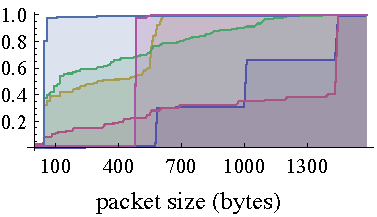
\includegraphics[width=1.7in]{size_cluster_examples}%
\label{fig:cluster-examples-size}}
\subfloat[example time clusters]
{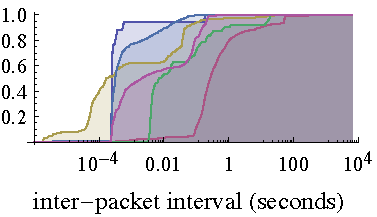
\includegraphics[width=1.7in]{time_cluster_examples}%
\label{fig:cluster-examples-time}}
\end{center}
\vspace{-0.3em}
\caption{{\footnotesize{CDF}}s of example flowlet clusters for size and time.}
\label{fig:cluster-examples}
\vspace{-1.35em}
\end{figure}

This first stage of \caps{PCA} extracts the common behavior across clusters into the matrix $R_{st}$, thereby allowing each flow's behavior to be expressed in terms of fewer cluster-like vectors. Common linear structure across all of the flows, however, may still exist. Before proceeding, we center each column by subtracting its mean: let $\mu_j = \frac{1}{f}\sum_{i=1}^{f}{F'_{ij}} \in \R^{b_s+b_t}$ and define $F''_{ij}=F'_{ij}-\mu_j$. We use \caps{PCA} again to find a set of basis vectors for the rows of $F''$ such that only 1\% of the variance in behavior across flows is lost. Let $a \in \N$ be the number of basis vectors required, and let $R_x \in \R^{(b_s+b_t) \times a}$ be the corresponding rotation matrix (its rows are the new basis vectors with respect to the old coordinates). We can then transform the set of flows one final time: $F''' = F'' R_x \in \R^{f \times a}$. Each row of this matrix still corresponds to a single original flow, but the coordinates are now a linear transformation of the original $c_s+c_t$ cluster coefficients onto only $a$ dimensions. The new coordinates are uncorrelated and explain the total variance of the flow behaviors in order of decreasing significance.

%The second application of \caps{PCA} is across the set of flow behaviors found in the trace data. Each flow is decomposed into flowlets, each of which belongs to a cluster. The flow-cluster matrix captures the fraction of each flow's packets that fall into each cluster. The matrix contains a row for each flow, and a column for each time and size cluster. The number of columns is greatly reduced after the first application of \caps{PCA}, since instead of needing a column for every cluster, only a column for every basis vector is needed.\footnote{This change is easily effected as a matrix multiplication by a block diagonal matrix, whose blocks are time and size PCA-rotations, respectively.} The reduced flow-cluster matrix is the subject of the second round of \caps{PCA}. This time we find a basis for the set of cluster-mixtures across flows such that 99\% of the variance observed is captured. Each flow behavior can then be expressed as a small set of coefficients for these basis vectors. %These basis vectors, in turn each encode a mixture of time and size clusters, which express the distributions of packet sizes and inter-packet intervals for the flow.

% In technical terms, the subspace spanned by the first $k$ \caps{PCA} basis vectors is the $k$-dimensional subspace of the data set that exhibits maximal variance. Moreover, the approximation provided by the first $k$ dimensions of the \caps{PCA} representation is the $k$-dimensional linear approximation of the data with minimal mean-squared reconstruction error.

\section{Results \& Discussion}
\label{sec:results}
\label{sec:discussion}

\begin{figure}
\vspace{-0.5em}
\begin{center}
\subfloat[size components S1-4]
{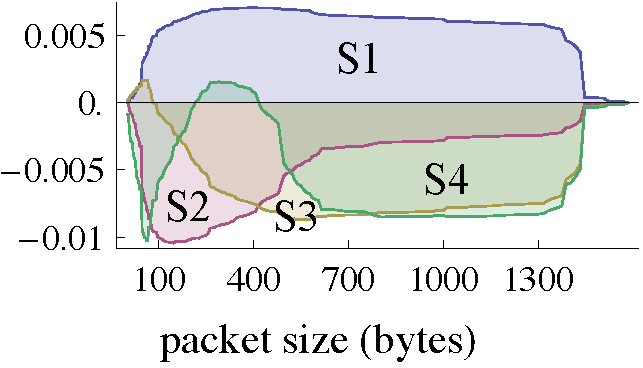
\includegraphics[width=1.7in]{size_principal_components}%
\label{fig:principal-components-size}}
\subfloat[time components T1-3]
{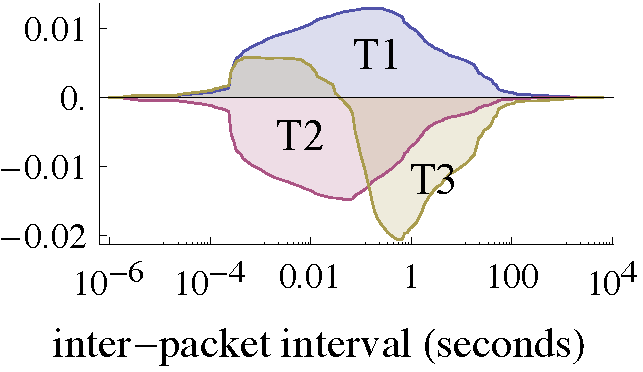
\includegraphics[width=1.7in]{time_principal_components}%
\label{fig:principal-components-time}}
\vspace{-0.3em}
\end{center}
\caption{Normalized {\footnotesize{CDF}} residuals for principal components of size and time behavior. The average {\footnotesize{CDF}} across all clusters is subtracted from each component's {\footnotesize{CDF}}. The difference is normalized so that the area between the residual and the $x$-axis is unity.}
\label{fig:principal-components}
\vspace{-1.4em}
\end{figure}

To test our methodology, we use traces recorded in an infrastructured 802.11g wireless \caps{LAN} with 18 access points, deployed at the 60th Internet Engineering Task Force meeting (\caps{IETF60}), held in San Diego during August of 2004. The details of how the trace was captured and processed can be found in \cite{Karpinski07:realism}~and~\cite{Karpinski07:cbr-failure}; a collection of application-level flow traces are extracted from raw \texttt{\small{tcpdump}} trace files. These flow traces provide the raw data for our analysis. We use the flows from a 210-minute subset of the full traces. This subset contains 4,138 flows, but we restrict our analysis to the 902 flows with at least 10 packets, since statistical tests such as \caps{BWS} lack adequate power for smaller samples than this.

Example size and time clusters, produced by the flow splitting and flowlet clustering algorithms, are shown in Figure~\ref{fig:cluster-examples}. These examples represent only six of each cluster type, out of 518 size clusters and 552 time clusters, but they give a sense of ``typical'' clusters.
%Most clusters capture a single, fairly simple set of values, but a fair portion of them capture more complex, mixed behavior.
%The output of the first round of \caps{PCA} on the collection of clusters is shown in Figure~\ref{fig:principal-components}.
Only six size principal components (\caps{PC}s) and three time \caps{PC}s explain 99\% of the variation in their respective collections of cluster behaviors. The net effects of various size and time \caps{PC}s on behavior distributions are illustrated in Figure~\ref{fig:principal-components}.
%To illustrate their net relative effect, they are subtracted from the average \caps{CDF} of all clusters, to find the relative difference, and then normalized so that the total area between the component and the $x$-axis is unity.
The first size component, \caps{S1}, for example, increases the proportion of a broad range of mid-sized packets relative to very small and very large packets. As another more complex example, the third time component, \caps{T3}, increases the proportion of smaller inter-packet intervals while drastically reducing the proportion of large ones. %In plain words, flows with large \caps{T3}-coefficients have frequent packets; flows with negative \caps{T3}-coefficients, on the other hand, tend to have infrequent packets.

\begin{figure}[b]
\vspace{-2em}
\begin{center}
\subfloat[{\footnotesize{S1}} \textit{vs.} {\footnotesize{S2}}]
{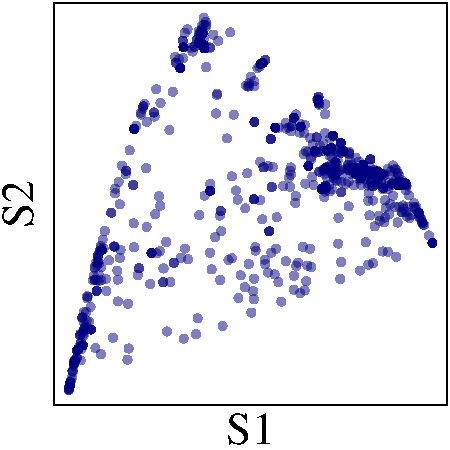
\includegraphics[width=1.125in]{scatter_plot_S1_S2.pdf}\label{fig:scatter-plot-S1-S2}}
\subfloat[{\footnotesize{T1}} \textit{vs.} {\footnotesize{T2}}]
{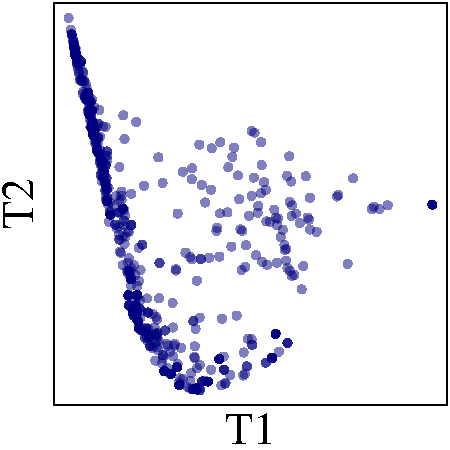
\includegraphics[width=1.125in]{scatter_plot_T1_T2.pdf}\label{fig:scatter-plot-T1-T2}}
\vspace{-0.3em}
\subfloat[{\footnotesize{S1}} \textit{vs.} {\footnotesize{T1}}]
{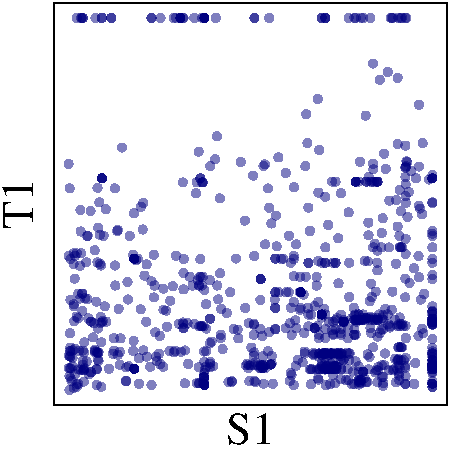
\includegraphics[width=1.125in]{scatter_plot_S1_T1.pdf}\label{fig:scatter-plot-S1-T1}}
\subfloat[{\footnotesize{X1}} \textit{vs.} {\footnotesize{X2}}]
{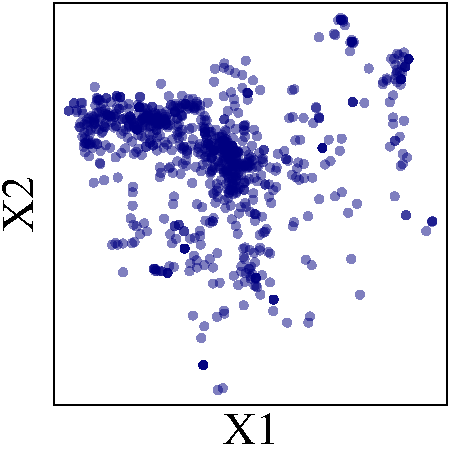
\includegraphics[width=1.125in]{scatter_plot_X1_X2.pdf}\label{fig:scatter-plot-X1-X2}}
\subfloat[{\footnotesize{X1}} \textit{vs.} {\footnotesize{X3}}]
{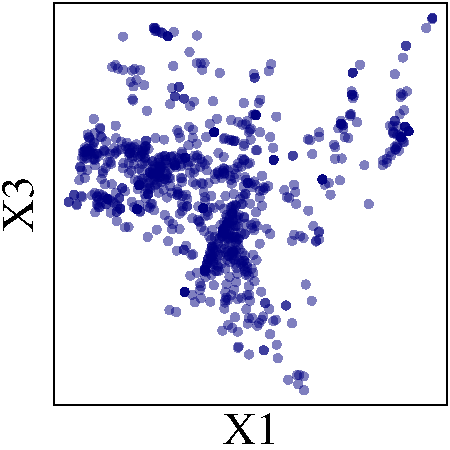
\includegraphics[width=1.125in]{scatter_plot_X1_X3.pdf}\label{fig:scatter-plot-X1-X3}}
\subfloat[{\footnotesize{X2}} \textit{vs.} {\footnotesize{X3}}]
{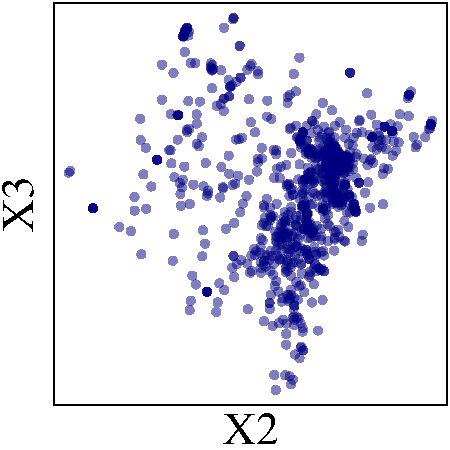
\includegraphics[width=1.125in]{scatter_plot_X2_X3.pdf}\label{fig:scatter-plot-X2-X3}}
\end{center}
\vspace{-0.3em}
\caption{Scatter plots of flow behaviors projected onto various pairs of time (\caps{T1-2}), size (\caps{S1-2}), and joint time-size (\caps{X1-3}) components.}
\label{fig:scatter-plots}
\vspace{-0.2em}
\end{figure}

\begin{figure*}
\vspace{-0.5em}
\begin{center}
\subfloat[flow behavior map --- {\footnotesize{S1}} \textit{vs.} {\footnotesize{T1}}]
{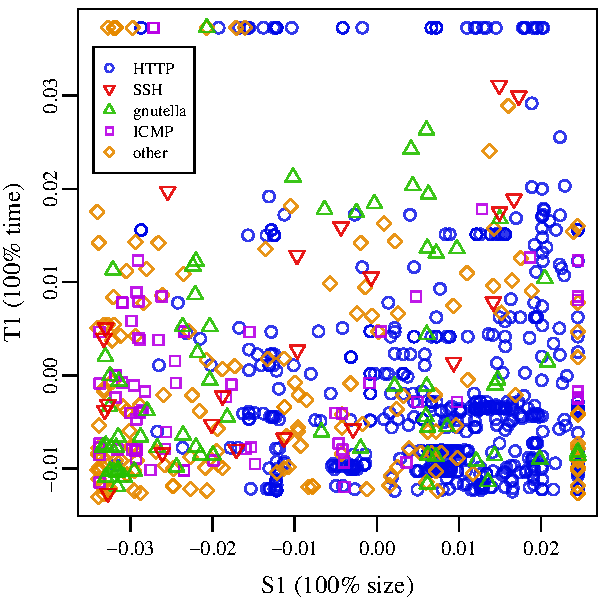
\includegraphics[width=2.878in]{flow_behavior_map_S1_T1}%
\label{fig:flow-behavior-map-S1-T1}}%
\hspace{0.05in}
\subfloat[flow behavior map --- {\footnotesize{X1}} \textit{vs.} {\footnotesize{X2}}]
{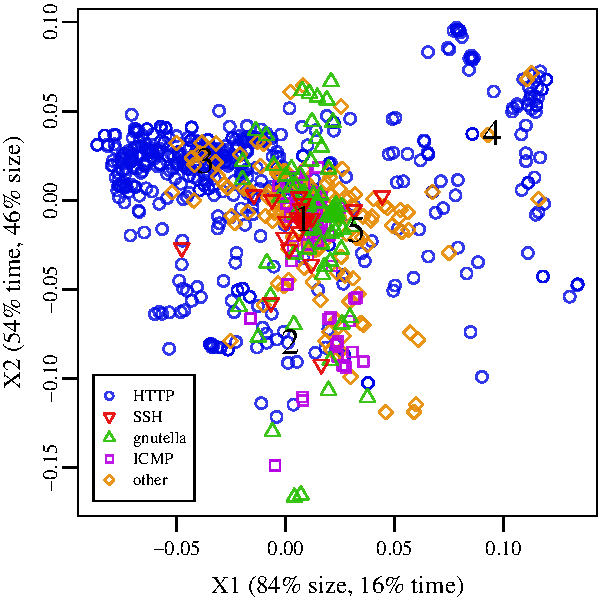
\includegraphics[width=2.878in]{flow_behavior_map_X1_X2}%
\label{fig:flow-behavior-map-X1-X2}}%
\hspace{0.05in}
\subfloat[clusters]
{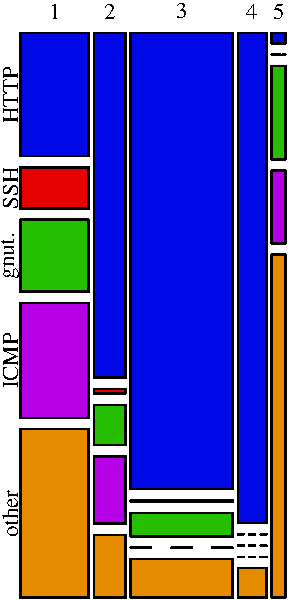
\includegraphics[width=1.195in]{traffic_cluster_mosaic}%
\label{fig:traffic-cluster-mosaic}}
\end{center}
\vspace{-0.4em}
\caption{Flows separated by application type projected onto the planes defined by two different pairs of principal behavior components. %---{\footnotesize{S1}} \textit{vs.} {\footnotesize{T1}} and {\footnotesize{X1}} \textit{vs.} {\footnotesize{X2}}.
Overlaid numbers in \ref{fig:flow-behavior-map-X1-X2} show the projected centroids of flow-behavior clusters (not to be confused with flowlet clusters) found in joint {\footnotesize{PCA}} space using standard $k$-means clustering. The relative sizes of the clusters and their composition are shown in \ref{fig:traffic-cluster-mosaic} as a mosaic plot.}
\label{fig:flow-behavior-maps} 
\vspace{-0.9em}
\end{figure*}

Since there are six size and three time \caps{PC}s after the first stage of \caps{PCA}, each flow can be represented in only nine dimensions. However, a great deal of structure remains in the interactions between the components, as seen in the scatter-plots in Figures~\ref{fig:scatter-plot-S1-S2}-\ref{fig:scatter-plot-S1-T1}. The plots map various pairs of coefficients for all the flows in our data set. While the \caps{PCA} produces linearly uncorrelated values, Figures~\ref{fig:scatter-plot-S1-S2}~and~\ref{fig:scatter-plot-T1-T2} clearly show a high degree of non-linear interaction. In Figure~\ref{fig:scatter-plot-S1-T1}, on the other hand, the size and time behaviors appear mostly independent. The non-linear patterns in Figures~\ref{fig:scatter-plot-S1-S2}~and~\ref{fig:scatter-plot-T1-T2} bear further attention. The curved portion of the convex hull of each pattern is approximately where vectors of the form {\small{$(0,\dots,0,1,\dots,1)$}} are mapped by the change of basis rotation. The other points can be written approximately as weighted sums of points on the hull in all \caps{PC} dimensions (in two dimensions, it must be true by the definition of convexity).

After the second round of \caps{PCA}, the nine separate size and time dimensions are mapped onto eight joint dimensions, each of which is partially time-like and partially size-like. These joint components can recreate 99\% of the variance in the original time and size components. Moreover, they are uncorrelated, normalized, and each have zero mean. Figures~\ref{fig:scatter-plot-X1-X2}-\ref{fig:scatter-plot-X2-X3} show scatter plots of the first three joint components, \caps{X1}, \caps{X2}, and \caps{X3}, against each other. The striking non-linear interactions that are so apparent in Figures~\ref{fig:scatter-plot-S1-S2}~and~\ref{fig:scatter-plot-T1-T2} are no longer evident, although some degree of visible dependence remains.
%Of course, since the transformation from size and time components to joint components is linear, the non-linear dependence cannot have simply ``vanished''; rather, the dependence has been shifted into the less significant components.
This is a significant improvement since we can approximate the distribution of the most significant joint components more readily with less dependence between the higher \caps{PC}s.

As an application of our methodology, we now consider how different traffic types are mapped onto various traffic behavior components. The major types of traffic found in the \caps{IETF60} trace are \caps{HTTP}, \caps{SSH}, gnutella, and \caps{ICMP}. Figure~\ref{fig:flow-behavior-maps} shows two different behavior maps. Figure ~\ref{fig:flow-behavior-map-S1-T1} uses \caps{S1} and \caps{T1} as coordinates, while Figure~\ref{fig:flow-behavior-map-X1-X2} uses \caps{X1} and \caps{X2}. Each view has its advantages. The coordinates of the size-time map have intuitive interpretations, given by the behaviors associated with components \caps{S1} and \caps{T1}. For example, flows in the lower-right portion of the plot have mid-sized packet sizes and inter-packet intervals that tend to be either very large or very small. This is consistent with the dominance of \caps{HTTP} traffic in this region: the small packets are \caps{TCP} setup and tear-down messages and \caps{GET} requests, while the larger packets are \caps{HTTP} responses.

The joint \caps{PCA} map has no such immedate interpretation, since the components \caps{X1} and \caps{X2} are linear combination of many time and size components. On the other hand, in the joint map, natural clusters of flow types emerge. Moreover, standard multi-dimensional analysis techniques can be applied to the full \caps{PCA} space. The overlaid numbers in Figure~\ref{fig:flow-behavior-map-X1-X2} mark the centroids of five clusters found using $k$-means clustering on the rows of $F'''$. %Figure~\ref{fig:traffic-cluster-mosaic} shows a mosaic plot of clusters versus traffic types. %\footnote{The width of each column is proportional to the number of flows in that cluster, while the height of each bar in a column is proportional to proportion of the flows in the cluster of that traffic type. As a result, the size of each box is proportional to the number of flows in that cluster of that type.}
Even though the clusters are derived based only on the time-space behavior flows, clear patterns with respect to traffic types emerge.
%This type of behavioral clustering provides a meaningful alternative to the traditional approach of categorizing traffic by application type.

Once the matrices $T,S,R_{st},R_x$ and the vector $\mu$ have been derived from a collection of traffic traces, new flows can be quickly and easily mapped into the size-time or joint \caps{PCA} spaces. First, quantize the empirical \caps{CDF} of the flow's packet size and inter-packet interval values using the method described in Section~\ref{sec:pca}. Let $x_s, x_t \in \R^n$ be the quantized \caps{CDF} vectors for size and time, respectively. Next, find coefficient vectors $\beta_s \in \R^{b_s}$ and $\beta_t \in \R^{b_t}$ that minimize the quantities
\begin{align}
\left\| S R_s \beta_s - x_s \right\|
\text{ and }
\left\| T R_t \beta_t - x_t \right\|.
\end{align}
Here $\left\|\,\cdot\,\right\|$ denotes the standard Euclidean norm. This is a linear sum-of-squares minimization problem, which can be solved quickly and efficiently by any numerical linear algebra system. Note that the matrices $SR_s$ and $TR_t$ can be pre-computed. The vectors $\beta_s,\beta_t$ already give us our size and time representations of the flow. Let $\beta = (\beta_s,\beta_t) \in \R^{b_s+b_t}$. To transform into joint \caps{PCA} space, we simply subtract $\mu$ and right-multiply by $R_x$: $\alpha = \left(\beta-\mu\right) R_x$.
The vector $\alpha$ is the joint \caps{PCA} representation of the flow. On modern computers, these vector and matrix operations are extremely fast, allowing us to produce dynamic flow behavior maps in real time. This capability could be extremely useful for network monitoring or anomaly and attack detection.

\begin{figure}
\vspace{-0.5em}
\begin{center}
\subfloat[size --- real]
{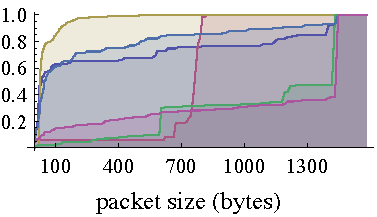
\includegraphics[width=1.7in]{size_flows_actual}}
\subfloat[time --- real]
{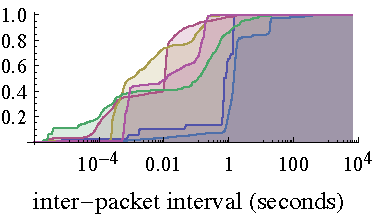
\includegraphics[width=1.7in]{time_flows_actual}}\vspace{-0.05in}
\subfloat[size --- generated]
{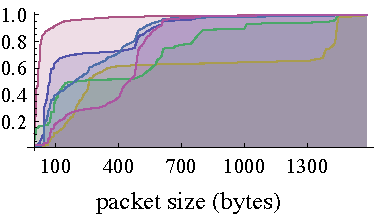
\includegraphics[width=1.7in]{size_flows_generated}}
\subfloat[time --- generated]
{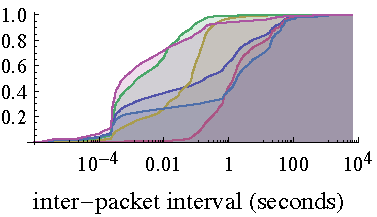
\includegraphics[width=1.7in]{time_flows_generated}}
\caption{Random flow behaviors --- real and generated.}
\label{fig:random-flows}
\end{center}
\vspace{-2em}
\end{figure}

Finally, we turn to the problem of generating realistic collections of flow behaviors. The coordinates of flows in joint \caps{PCA} space can be very roughly approximated as a multivariate normal distribution, since the coordinates are uncorrelated and have zero means. This approximation is very rough, and not remotely statistically rigorous, but still, very useful---and possibly just good enough. Using this rough model, we can generate random multivariate normal deviates in joint \caps{PCA} space and reverse transform them to get semi-realistic flow behaviors. Explicitly, if $\alpha^* \in \R^a$ is a randomly generated joint \caps{PCA} vector, then we can transform it via matrix inversion:
\begin{align}
(\gamma^*_s,\gamma^*_t) &= \left(\alpha^* R_{x}^{-1}+\mu\right) R_{st}^{-1} \in \R^{c_s+c_t}.
\end{align}
The vectors $\gamma^*_s,\gamma^*_t$ are relative weights for size and time cluster atoms. Negative weights are artifacts of imperfect dependence modeling and should simply be ignored. The actual size and time \caps{CDF}s are produced from $\gamma^*_s$ and $\gamma^*_t$ (after fixing up) via left-multiplication by the matrices $S$ and $T$. Alternately, the actual empirical \caps{CDF} for each cluster can be randomly sampled, and the weights used to chose randomly between the clusters. Figure~\ref{fig:random-flows} compares six randomly selected real flow behaviors with six random synthetic flows generated using this method. The resemblance is fairly good. While this method is somewhat rough, no other method currently exists for generating realistic full-network collections of flow behaviors based on real trace traffic. %However, some deficiencies are already clear. The perfect independence of $\alpha^*$ translates into more evenly distributed mixing of clusters than is found in real flows. This results in generated flows being smoother and more homogeneous than real flows.
It remains to be seen if the realism of flows generated this way is sufficient by the standards defined in~\cite{Karpinski07:realism}~and~\cite{Karpinski07:cbr-failure}. We intend to investigate precisely this question in our future research.

\section{Conclusions \& Future Work}
\label{sec:conclusions}

This paper presents a fundamentally different way of viewing and understanding network trace data. The most radical concept entailed in this approach is that of finding common ``atoms'' of flow behavior and using these as the basis for representing and analyzing network-wide traffic patterns. The statistical and algorithmic methodology for finding these atoms of behavior is a significant contribution in itself, with application well beyond the field of traffic analysis. Once the atoms of behavior are extracted, it becomes natural to view the space of behaviors as a vectors space generated by these units. This representation puts a vast array of powerful linear algebraic tools at our disposal for understanding and analyzing network traffic. We have only begun to scratch the surface of the possible applications of this atomic theory of flow behavior.

%\section{Acknowledgments}
%{\small
%This work was funded in part by \caps{NSF} Career Award \caps{CNS-0347886} and by \caps{NSF} \caps{NeTS} Award \caps{CNS-0435527}. Special thanks to Matthew Allen, Khaled Harras, Allan Knight, and Rich Wolski for their invaluable help and advice.
%}
\bibliography{IEEE,references}

\end{document}
